\documentclass[tikz]{standalone}
\usetikzlibrary{patterns}
\usetikzlibrary{shapes,arrows}
\usetikzlibrary{decorations.pathreplacing, positioning}
\definecolor{greengreen}{rgb}{0.0, 0.42, 0.24}
\definecolor{calpolypomonagreen}{rgb}{0.12, 0.3, 0.17}
\definecolor{forestgreen}{rgb}{0.13, 0.55, 0.13}

\begin{document}
\noindent
  
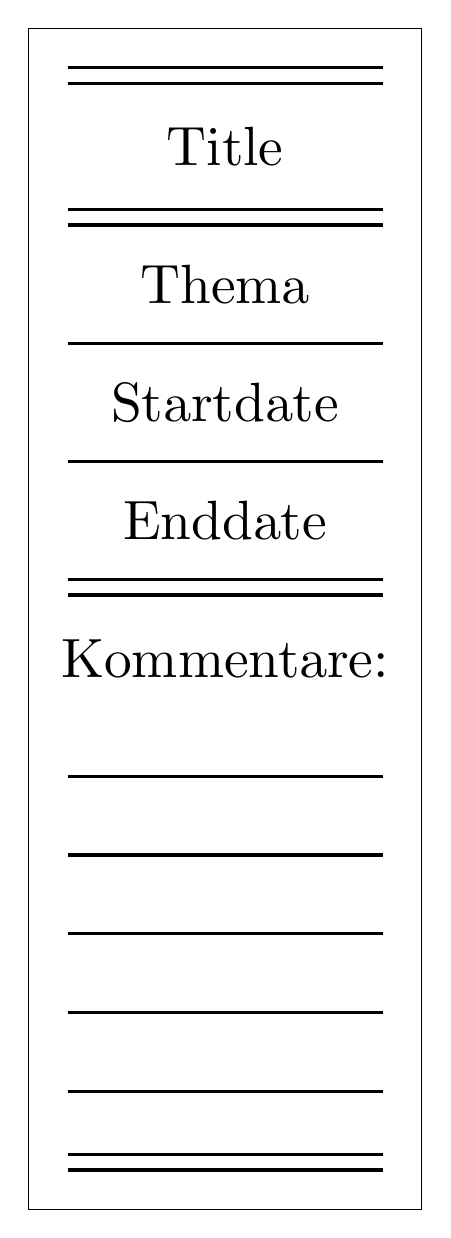
\begin{tikzpicture}

  % INPUT: Title
  \node[scale=2, align=center] at (2.5,13.5) {Title};

  % INPUT: Subject
  \node[scale=2, align=center] at (2.5,11.75) {Thema};
  \node[scale=2, align=center] at (2.5,10.25) {Startdate};
  \node[scale=2, align=center] at (2.5,8.75) {Enddate};

  % Kommentare

  \node[scale=2, align=center] at (2.5,7) {Kommentare:};

  % Background  
  \draw (0,0) -- (0,15) -- (5,15) -- (5,0) -- cycle;

  % Decoration
  \foreach \x in {0,0.2, 1.8,2, 3.5, 5, 6.5,6.7, 9,10,11,12,13, 13.8,14}
    \draw[very thick] (0.5,14.5 - \x) -- (4.5,14.5 - \x);

  \end{tikzpicture}%
\end{document}
